\subsubsection{In Situ Process Monitoring and Feedback}
\begin{figure*}
	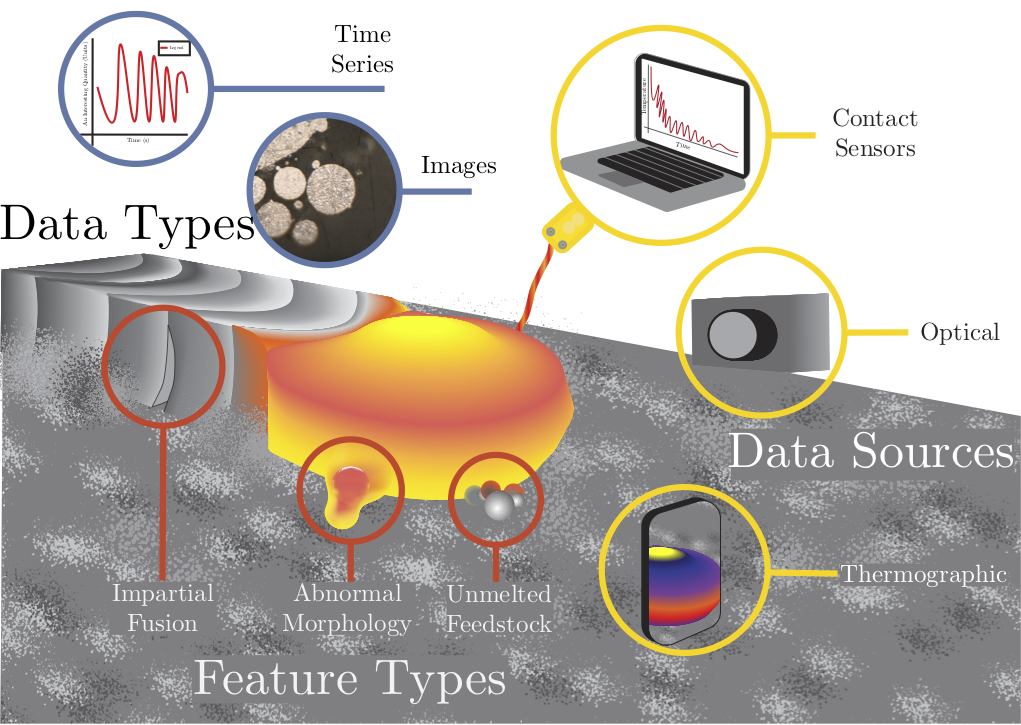
\includegraphics[width=0.85\linewidth]{Images/melt_pool}
	\caption{A few examples of data types, data sensors, and features to detect in a laser powder bed fusion manufacturing process. The wide range of signals to monitor then control makes feedback and control in AM especially difficult. Computer vision techniques can be applied to automatically detect features of interest across multiple data types and data sensor simultaneously.}
	\label{fig:melt_pool}
\end{figure*}

In situ monitoring, feedback, and control has been consistently ranked as one of the most-needed technologies for advancing additive manufacturing \cite{Berumen2010, Tapia2014, Mani2017}. The combination of rapid solidification and the small length scales of AM solidification can make traditional process monitoring approaches difficult. Furthermore, there are many processes/problems to monitor for during the manufacturing process, with equally as many sensor types for monitoring as shown in Figure \ref{fig:melt_pool}. Machine learning can fill in gaps where human-specified process monitoring models are insufficient.

Process monitoring involves acquisition of real-time signals which can reveal information about a wide variety of phenomenon during manufacturing. Most studies utilizing in situ processing monitoring are focused on identifying a) important indicators of microstructure development; or b) deviations from the normal process that cause defect formation. McKeown et al. has used dynamic transmission electron microscopy to measure solidification rates in powder bed AM \cite{McKeown2016}. Bertoli et al. has also characterized cooling rates using high speed imaging \cite{Bertoli2017}. Raplee et al. has used thermography to monitor the solidification and cooling rates of electron beam powder bed fusion, relating the temperature profiles to defect and microstructural characteristics \cite{Raplee2017}. Distortion of parts due to thermal cycling was investigated by Denlinger et al. by means of thermocouples in contact with the build substrate \cite{Denlinger2015}. 

Traditional feedback and control for manufacturing involves human-identified signatures/errors in measured signals. A basic feedback and control system is the proportional-integral-derivative (PID) controller that, in its most basic application, measures signal error from an expected mean and provides feedback to correct for deviations. Additive manufacturing has so many signals to simultaneously monitor that a desired `mean' function may not be obvious to define. A more adaptable identification and feedback method is machine learning and, specifically, computer vision. Computer vision can be employed in additive manufacturing to monitor and characterize temperature profiles, identify abnormal melt pool morphologies, and automatically detect defect formation. 

The type of data being collected in situ is most often in the form of time series or image data. In computer vision, as with traditional feedback and control, algorithms are used to identify deviations from a desired signal. The power of computer vision approaches are their ability to simultaneously monitor and identify signal changes across multiple sensor types, as well as multiples different types of deviation from a single sensor. Examples include identifying a spike in temperature or a sharp change in intensity in an image indicating a deviation from a desired processing conditions. Image processing \textit{filters} can be used to selectively modify or extract features AM data. Image processing filters are mathematically analogous to those introduced for topology optimization (Section~\ref{sec:topology optimization}).

A filter is implemented as a mathematical operation, a kernel, applied to a window of time series data or an area of pixels in an image. For images, filters attempt to use local spatial information and \textit{a priori} knowledge of the expected properties of the image to improve image quality and extract features, e.g., distinctive characteristics such as edges or regions of similar intensity (domains) that represent the boundaries or spatial extents of objects, phases, etc. 

The small length scale of AM processes (relative to most detector coverage areas) as well as the fast solidification rates causes low signal-to-noise ratios in AM signals. As such, filters are often selected to reduce noise in the raw signal, or identify transitions between visually distinct regions, such as the transition between melt pool and powder bed. A comprehensive review of image filters is beyond the scope of this review, so the interested reader is directed to the many works on this topic, c.f.,~\citet{Vernon1991}. However, three use cases are especially common and worth specific acknowledgement: reduction of high-frequency noise, also known as salt-and-pepper noise; additive noise reduction; and edge detection.

High frequency noise is characterized by sudden changes in intensity relative to the surrounding field. Although there are a number of possible causes, this may be caused by pixel-level variability or insufficiency in the detector, e.g. ``dead pixels'' or excessive gain. Median and conservative filters are commonly used when the fraction of noise pixels is large (1\%--10\%) and small ($<$ 1\%), respectively.

Additive noise, unlike high frequency noise, is a result of insufficient Poisson (counting) statistics, which may result from insufficient incident intensity, exposure time, or detector efficiency, random variability in the intensity of the input signal (Gaussian noise), or both. A gaussian filter adjusts the intensity of each pixel according to the gaussian-weighted intensities of neighboring pixels. Unlike median and conservative filters, a gaussian filter will soften edges, making adjacent domains less distinct.

Filters also have applications beyond noise reduction, primarily in object and feature detection. Detecting phenomena of interest during manufacturing is the first step to feedback and control mechanisms. Edge detection captures local changes in intensity to identify transitions between adjacent domains. In noisy images filters like the Laplacian or Laplacian of Gaussian generally identify many spurious edges and are often used as part of a larger algorithm, such as Canny edge detection~\cite{Canny1986}. The Canny edge detection algorithm has uses in identifying the boundary between a melt pool and a powder bed, monitoring shape deviation due to thermal stresses, and identifying boundaries of unintended objects in an image, such as an unmelted powder particle inclusion. 

The Canny edge detector, among other edge detection algorithms, can \textit{identify} boundaries in an image, but not necessarily classify them. Classification of identified features is where machine learning processes are useful. The use of filters alone does not constitute machine learning, but features extracted using these filters can be used as part of the larger machine learning workflow. For example, these features can be used in learning algorithms to correlate characteristic features with particular behaviors in the manufacturing process. In this case, identification of a feature, or set of features, may be sufficient to indicate a particular process outcome.

A computer vision method called \textit{template matching} can be used for automatic identification of signal features. Template matching involves the comparison of measured features to a database of pre-identified signal features. For an AM case, template features would be abnormal melt pool morphologies, inclusion of unmelted powder particles, denudation near the melt zone, and the like. The scale-invariant feature transform (SIFT) \cite{Lowe2004} and a variant, ``Speeded-Up Robust Features'' (SURF) \cite{Bay2008} are both feature identification algorithms that can be used for template matching. Another template matching algorithm is the \textit{bag of visual words} or dictionary method~\cite{DeCost2015}. A collection (dictionary) of typical features from the AM process can be built based on features obtained from filters. The features measured in situ are compared with dictionary entries. If an in situ feature matches a defect-indicative feature from the dictionary, then it is likely a defect has formed during manufacturing.

\begin{figure*}
	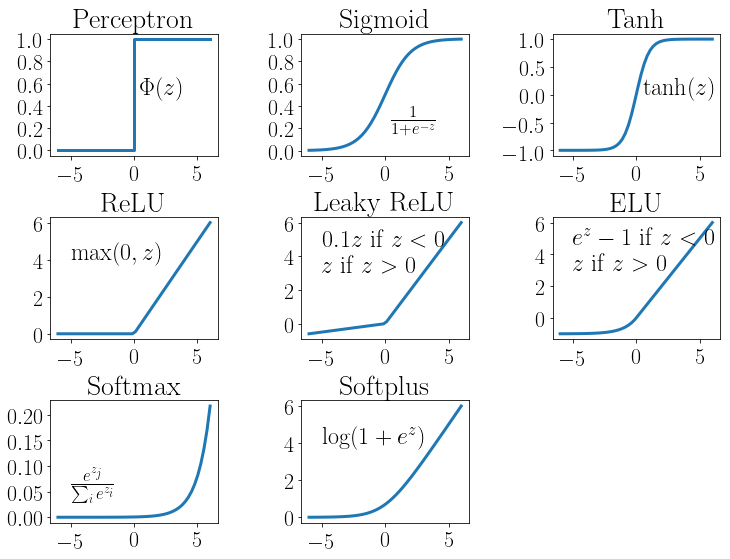
\includegraphics[width=0.85\linewidth]{Images/ActivationFunctions}
	\caption{Common activation functions in artificial neural networks (NNs) that introduce nonlinearity into the NN. The sigmoid is the archetype activation function because the closed form solution for the derivative of the sigmoid, which is used in backpropagation {\color{red} The reader does not know what backpropagation is}, is an excellent pedagogical tool; however, the rectified linear unit (ReLU) is, at present, the most common activation function in the hidden layers of NN. Uses for the other activation functions are provided in the text.}
	\label{fig:activation functions}
\end{figure*}

Neural networks (NNs) are particularly well-suited to handle features extracted from images, or simply the images themselves. There are many references that describe neural networks in detail, c.f.~\cite{Hastie2009}, and an increasing number that address the specific challenges associated with neural networks in materials science~\cite{Bhadeshia2009}. There are several properties of NNs that are worth repeating here, however. Each layer in a NN is connected to the next layer through an affine (linear) transformation. This step stretches, scales, and skews the input vector.
\begin{equation}
	{\bold z}^{(i+1)} = \boldsymbol \theta_i^T {\bold x}^{(i)}
\end{equation}
where ${\bold z}^{(i+1)}$ is the input into the $(i+1)$ layer and ${\bold x}^{(i)}$ is the output from the previous, $i^\textrm{th}$ layer. Then, an activation function, such as those summarized in Figure~\ref{fig:activation functions}, introduces a non-linearity that can warp/distort the vector input to that layer. 

\begin{equation}
	{\bold x}^{(i+1)} = f \left( {\bold z}^{(i+1)} \right)
\end{equation}

The model hyperparameters $\mathbf{\theta}_i^T$ are regression weights that associate outputs from each layer $\mathbf{x}^{(i)}$ to subsequent layers $\mathbf{z}^{(i + 1)}$. The benefit of stretching, skewing, and distorting vector inputs from each layer is elucidating object features which are strongly correlated with model outputs but may not be obvious from the original image or after the first filter application. A regression algorithm trained on only a dataset of melt pool boundaries may not transfer well to new images of melt pools because it is unlikely that any two melt pools look \textit{exactly} the same. However, repeated applications of affine transformation can bring about features that are common to all melt pools but may not be obvious to the human eye. In a process as complicated as AM identification of high level features through these transformations will make feature identification possible despite the high variance in types of AM images.

By increasing the depth of the NN, that is, adding additional layers, and the width (number of nodes) of those layers, a NN can be used to approximate any function, making them powerful regression and classification tools~\cite{Hornik1989}. However, the general sparsity of materials data coupled to the complexity of process--structure--process relationship requires an understanding of the tradeoffs and requirements of using NNs in materials science, and in AM more specifically. Beyond the basics of model architecture, overfitting and the bias--variance tradeoff that is part of any machine learning model, a basic understanding of the role of activation functions can help to develop an intuition for the use of NN in materials and manufacturing.

One of the early uses of NNs was in classification. The perceptron, logistic sigmoid (or simply, sigmoid), and hyperbolic tangent are all activation functions that choose between two options (0 or 1, or in the case of $\tanh$, -1 or 1). Although more mathematically complicated than the perceptron, the logistic sigmoid,
\begin{equation}
	\sigma(z) = \frac{1}{1 + e^z}
	\label{sigmaz}
\end{equation}
has the beneficial property that its derivative is an analytical expression of the sigmoid function itself, i.e.
\begin{equation}
	\sigma^\prime(z) = \sigma(z) \left( 1 - \sigma(z) \right)
	\label{sigmaprime}
\end{equation}
which enables very quick calculation of the Jacobian during backpropagation {\color{red} We either need to fully explain what backpropogation is, or simplify this discussion into essentially saying `they help with fitting model weights' and skip the how of it.} and training, that is used to fit the layer weights, $\boldsymbol \theta_i$. While a binary option may seem overly limiting, even multinomial classification can be broken down into a sequence of such binary classificiations: \textit{A} or not \textit{A}; and if not \textit{A}, then \textit{B} or not \textit{B}; and if not \textit{B}, \textit{C} or not \textit{C}; etc. However, such a serial solution will require more layers and, with more layers, longer training on larger datasets in order to fit all model hyperparameters.

In the case of a multinomial classification problem, a more simple network may be possible by using one-hot encoding. A one-hot encoding vector is defined for $N$ exclusive options: one element in the $N$-element vector is 1, all other values are 0. Rather than using multiple layers to construct the binomial ladder required to simulate a multinomial decision, the softmax activation function selects one-from-many in a single layer. Since each value in the input vector appears in the softmax exponent, even small differences in the magnitude of $z$ result in large differences in the output of this activation function; one option, represented by one node or neuron in the layer, dominates. Simplification of the network architecture by choosing activation functions that more closely resemble the nature of the problem is one point where domain-specific knowledge is critical.

NN are also used for regression. Unlike classification, regression requires a continuously variable response across the problem domain, and so the binary posit of the logistic sigmoid and the multinomial posit of the softmax are replaced with activation functions such as exponential linear unit (ELU), softplus, Leaky ReLU, and most commonly, ReLU, the Rectified Linear Unit. Visual examples of these activation functions can be seen in Figure \ref{fig:activation functions}. While each behaves differently, particularly across the negative domain ($x < 0$), the simplicity and robustness of the ReLU have made it the most commonly used activation function for regression-type layers.

Combining the concepts of neural networks and image processing filters, convolutional neural networks (CNNs) not only learn how to correlate features to results, they are specifically designed to identify the filters that extract those features. These networks require large numbers of hyperparameters, in the tens to hundreds of millions, which introduces an insurmountable training burden due to the sparsity of materials data. However, CNNs trained on natural images have demonstrated a remarkable similarity in their initial layers~\cite{Yosinski2014}. These first few layers identify basic shapes, edges, and colors that are common to many image types; a phenomenon that many groups have exploited overcome the limitation of data sparsity through transfer learning~\cite{Ling2017a}, including specific work in the field of additive manufacturing. Yuan et al \cite{Yuan2018} were able to successfully monitor melt track width, standard deviation, and continuity of tracks in situ during laser powder bed manufacturing. Scime and Beuth trained a convolutional neural network to identify six different types of defect which are typical of laser powder bed fusion, with fairly good prediction accuracy \cite{Scime2018}. Kwon et al. classified melt pool morphologies using a neural network \cite{Kwon2018}. These studies encompass only a few of the possibilities of in situ process monitoring for AM. 



